\chapter[Proposta]{Proposta}

Este capítulo apresenta detalhes sobre a pesquisa realizada durante o desenvolvimento do TCC\_1 e do TCC\_2. O capítulo foi organizado nas seções de \textit{Obtenção da base teórica}, a partir da utilização de revisão sistemática, e \textit{Adaptação e implementação}, onde serão especificados os objetivos práticos da pesquisa.

\section{Obtenção da base teórica} % (fold)
\label{sec:obtenção_da_base_teórica}
	
	Como qualquer trabalho científico, para alcançar os objetivos da pesquisa, faz-se necessária a realização de uma pesquisa bibliográfica buscando obter uma base teórica suficiente para sustentar o trabalho realizado. Durante este trabalho de conclusão de curso, como uma forma de obtenção da base teórica, foi utilizada a técnica de revisão sistemática.

	O grande foco da revisão sistemática tem sido as técnicas de resolução do problema de SLAM utilizadas atualmente, em diferentes contextos. Vale ressaltar que o foco será na utilização das mesmas em um contexto simplificado e educacional. A identificação destas técnicas possibilita a seleção e adaptação das mesmas para viabilizar sua implementação no contexto simplificado da robótica educacional.

	A revisão sistemática desenvolvida durante esta etapa se encontra detalhada na seção \ref{sec:revisão_sistemática}, onde são apresentados deste o planejamento da revisão ate a condução e divulgação dos resultados da mesma. A seção \ref{sec:adaptação_e_implementação} irá apresentar detalhes referentes ao objetivo prático deste trabalho. Para alcançar estes objetivos, serão utilizados insumos obtidos durante a obtenção da base teórica, a partir da revisão sistemática.

% section obtenção_da_base_teórica (end)

\section{Adaptação e implementação} % (fold)
\label{sec:adaptação_e_implementação}

	Com a identificação e análise das diferentes técnicas de resolução do problema de SLAM, fruto da revisão sistemática, serão realizadas provas de conceito ao início da segunda etapa do trabalho. Estas provas de conceito têm como objetivo selecionar, primeiramente, qual filtro probabilístico será utilizado neste trabalho.

	De acordo com o resultado obtido com a revisão sistemática, a grande maioria das soluções do problema de SLAM identificadas utilizam o filtro de Kalman, como mostra a tabela \ref{tab:resultadosRevisao}. Por outro lado, a utilização do filtro de partículas possibilita a implementação, com maior facilidade, do problema do sequestro do robô, como foi apresentado na seção \ref{sec:section_name}.

	Desse modo, a escolha do filtro a ser utilizado ainda depende de estudos mais específicos sobre a implementação dos mesmos, levando em consideração sua complexidade e suas vantagens em relação ao concorrente.

	Ao final deste trabalho, espera-se obter uma solução onde o robô seja inserido em um ambiente desconhecido, em um ponto desconhecido e, a partir das informações obtidas pelos sensores, o mesmo construa um mapa do local, utilizando este mesmo mapa, simultaneamente para se auto-localizar no ambiente. Para isso, estarão disponíveis os sensores de distância (sonar), odométricos e, possivelmente, uma bússola.

	Como as técnicas identificas durante a revisão sistemátia utilizam, em sua maioria, sensores como \textit{câmera de vídeo} e sensores a \textit{laser}, adaptações serão necessárias para viabilizar a resolução do problema com a utilização dos sensores citados anteriormente (sonar, odometria e bússola).

	A resolução do problema será realizada de maneira simplificada, possibilitando sua conclusão durante o período previsto para o desenvolvimento da segunda etapa deste trabalho de conclusão de curso. Desse modo, questões referentes ao desempenho e máxima precisão não fazem parte do foco deste trabalho.

	A arquitetura da solução que será desenvolvida durante este trabalho segue o apresentado ao percorrer da revisão sistemática, como apresenta a figura \ref{img:arquitetura_mais_utilizada}. Nesta arquitetura, o robô é responsável apenas por obter as informações do ambiente, a partir de seus sensores, e \textit{odebecer} as ordens do computador. Já o computador, será responsável por processar as informações obtidas pelo robô e, a partir deste processamento, enviar decisões referentes à movimentação e localização ao robô. Esta arquitetura foi destacada, durante a revisão sistemática, como uma arquitetura de processamento remoto, onde nenhum processamento é feito localmente (no próprio robô), como apresenta a seção \ref{sub:arquitetura_solucao}.

	Durante as seções a seguir, serão apresentadas informações referentes à solução e desenvolvimento durante a segunda etapa deste trabalho.

	\subsection{Arquitetura do Robô} % (fold)
	\label{sub:arquitetura_do_robô}
		
		De acordo com \cite{vieira}, a arquitetura de robôs móveis pode ser sub-dividida cinco camadas: \textit{percepção}, \textit{decisão}, \textit{planejamento de caminho}, \textit{geração de trajetória} e \textit{sistema de controle}.

		A primeira camada, denominada \textit{camada de percepção}, será o grande foco deste trabalho, onde a identificação de obstáculos para mapeamento do ambiente é uma atividade essencial para a resolução do problema de SLAM. Esta camada é responsável por adquirir informações sobre o ambiente ao seu redor, viabilizando a navegação e auto-localização no mesmo.

		Já a segunda camada, \textit{decisão}, que foi o foco de trabalho de \cite{tccCarol}, tem como responsabilidade processar decisões do robô. Nesta camada se encontra o verdadeiro cérebro do robo, como afirma \cite{vieira}.

		Na terceira camada, \textit{planejamento de caminho}, será utilizado, como ferramenta de apoio, o \textit{framework} Traveller, desenvolvido por \cite{tccRodrigo}. Sua utilização se refere ao planejamento da navegação no ambiente após o mapeamento, mesmo que parcial, do ambiente. Ou seja, enquanto o robô navega e mapeia o ambiente, os locais já percorridos (conhecidos e mapeados) possibilitarão a utilização do \textit{framework}. Por outro lado, em locais ainda desconhecidos, o planejamento do caminho será feito de forma aleatória, buscando mapear o ambiente como um todo.

		A quarta camada, \textit{geração da trajetória}, utiliza o planejamento realizado na camada anterior para definir quais açoes devem ser realizadas no \textit{hardware} do robô, levando em consideração as características físicas do mesmo. Com isso, a quinta camada, \textit{sistema de controle}, é chamada para verificar o recebimento adequado dos sinais, assim como sua execução nos atuadores. 

		A figura \ref{img:camadas} apresenta as cinco camadas, onde, no nível mais alto, se encontra a camada de percepção, que é o foco deste trabalho. 

		\begin{figure}[H]
			\centering
			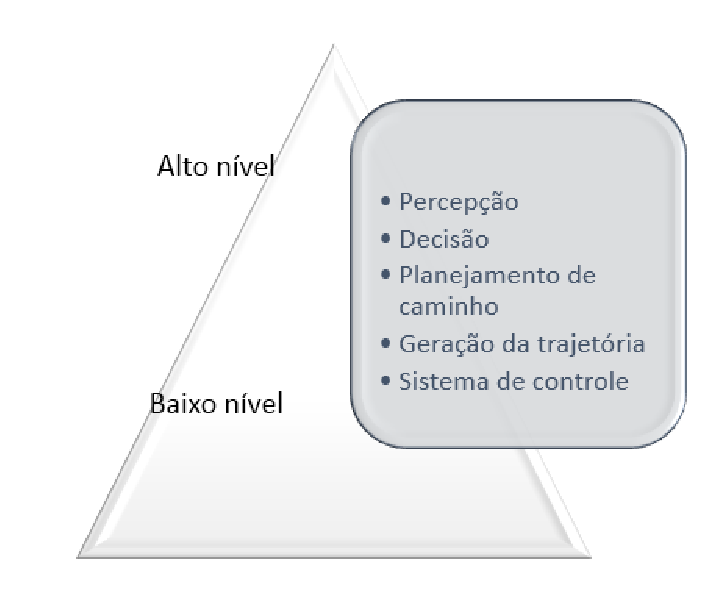
\includegraphics[scale=0.6]{figuras/camadas.eps}
			\caption[Arquitetura do robô]{Arquitetura do robô. Fonte \cite{vieira}.}
			\label{img:camadas}
		\end{figure}

	\subsection{Montagem do robô} % (fold)
	\label{sub:montagem_do_robô}
		
		A montagem utilizada durante o início deste trabalho, mais especificamente durante a realização da prova de conceito, é baseada em esteiras. O robô é equipado com um sonar, para identificar a distância de obstáculos, e um sensor de toque. Para movimentação, foram utilizados dois motores, A e B, dispostos na direita e esquerda, respectivamente. A Figura \ref{img:fotoRobo} apresenta a montagem utilizada.

		\begin{figure}[H]
			\centering
			\includegraphics[scale=0.25]{figuras/fotoRobo.eps}
			\caption[Montagem do robô]{Montagem do robô.}
			\label{img:fotoRobo}
		\end{figure}
	% subsection montagem_do_robô (end)

	\subsection{Ambiente utilizado} % (fold)
	\label{sub:ambiente_utilizado}
		
		A partir da realização da prova de conceito, durante a primeira etapa deste trabalho, a qual está descrita na seção \ref{sec:desenvolvimento_prático}, optou-se pela utilização de um ambiente com, no mínimo, dois metros quadrados de área disponível para navegação. Serão utilizados, durante a realização da segunda etapa deste trabalho, cômodos como quartos, salas ou escritórios para implementação da solução proposta.

		Inicialmente o ambiente proposto se baseava no tapete de missões \textit{Nature's Fury}, com uma área pequena o suficiente para que os erros impactassem bastante no resultado do mapeamento. Isto ocorre devido a característica específica do sensor de distância utilizado, que está descrita de forma clara na seção \ref{sub:características_técnicas}.

		Com a utilização de ambientes com uma área maior, espera-se que o impacto destes erros não seja tão problemático quanto em ambientes pequenos, como o utilizado na prova de conceito. Dentro do ambiente serão adicionados obstáculos além das paredes que contornam o ambiente, possibilitando testes com maior qualidade e eficiência.


	% subsection ambiente_utilizado (end)

	\subsection{Condução do trabalho} % (fold)
	\label{sub:condução_do_trabalho}

		O desenvolvimento deste trabalho terá como base, durante o TCC\_2, a metodologia ágil, utilizando o conceito de \textit{releases}, \textit{sprints} e \textit{histórias} para apoiar o mapeamento e gerenciamento dos requisitos, assim como o acompanhamento da evolução do trabalho ao longo do tempo. Para representar as \textit{releases}, \textit{sprints} e \textit{histórias}, serão utilizadas, respectivamente, as ferramentas de criação de \textit{tags}, \textit{milestones} e \textit{issues} presentes no GitHub\footnote{https://github.com}.

		Com o objetivo de acompanhar o desenvolvimento, a ferramenta \textit{waffle.io}\footnote{https://waffle.io}, em integração com o GitHub, será utilizada. Possibilitando maior visibilidade e organização do \textit{status} do trabalho.

		Ao início de cada \textit{sprint}, serão analisadas as histórias que farão parte da mesma, levando em consideração o \textit{velocity} do pesquisador e o período fixo para cada \textit{sprint} de duas semanas. Ao final de cada \textit{sprint}, o \textit{velocity} deverá ser atualizado para melhor acompanhamento do projeto.

		De acordo com a utilização do conceito de \textit{velocity}, as histórias deverão ser pontuadas a partir de sua complexidade de implementação, em relação ao conhecimento do desenvolvedor. A pontuação será realizada ao início de cada \textit{sprint}.

		A gerência de configuração e versionamento de todo o trabalho se baseia na utilização da ferramenta GitHub, baseada em projetos GIT. Desse modo, para organização dos artefatos do trabalho, foi criada uma Organização\footnote{https://github.com/SlamProblemTcc} no GitHub, a qual possui dois repositórios, um referente ao versionamento de toda a documentação do projeto\footnote{https://github.com/SlamProblemTcc/slam\_lego\_doc} (\textit{slam\_lego\_doc}), e um referente ao versionamento do código\footnote{https://github.com/SlamProblemTcc/slam\_lego} (\textit{slam\_lego}). A Figura \ref{img:github} apresenta a organização utilizada para versionamento deste trabalho.

		\begin{figure}[H]
			\centering
			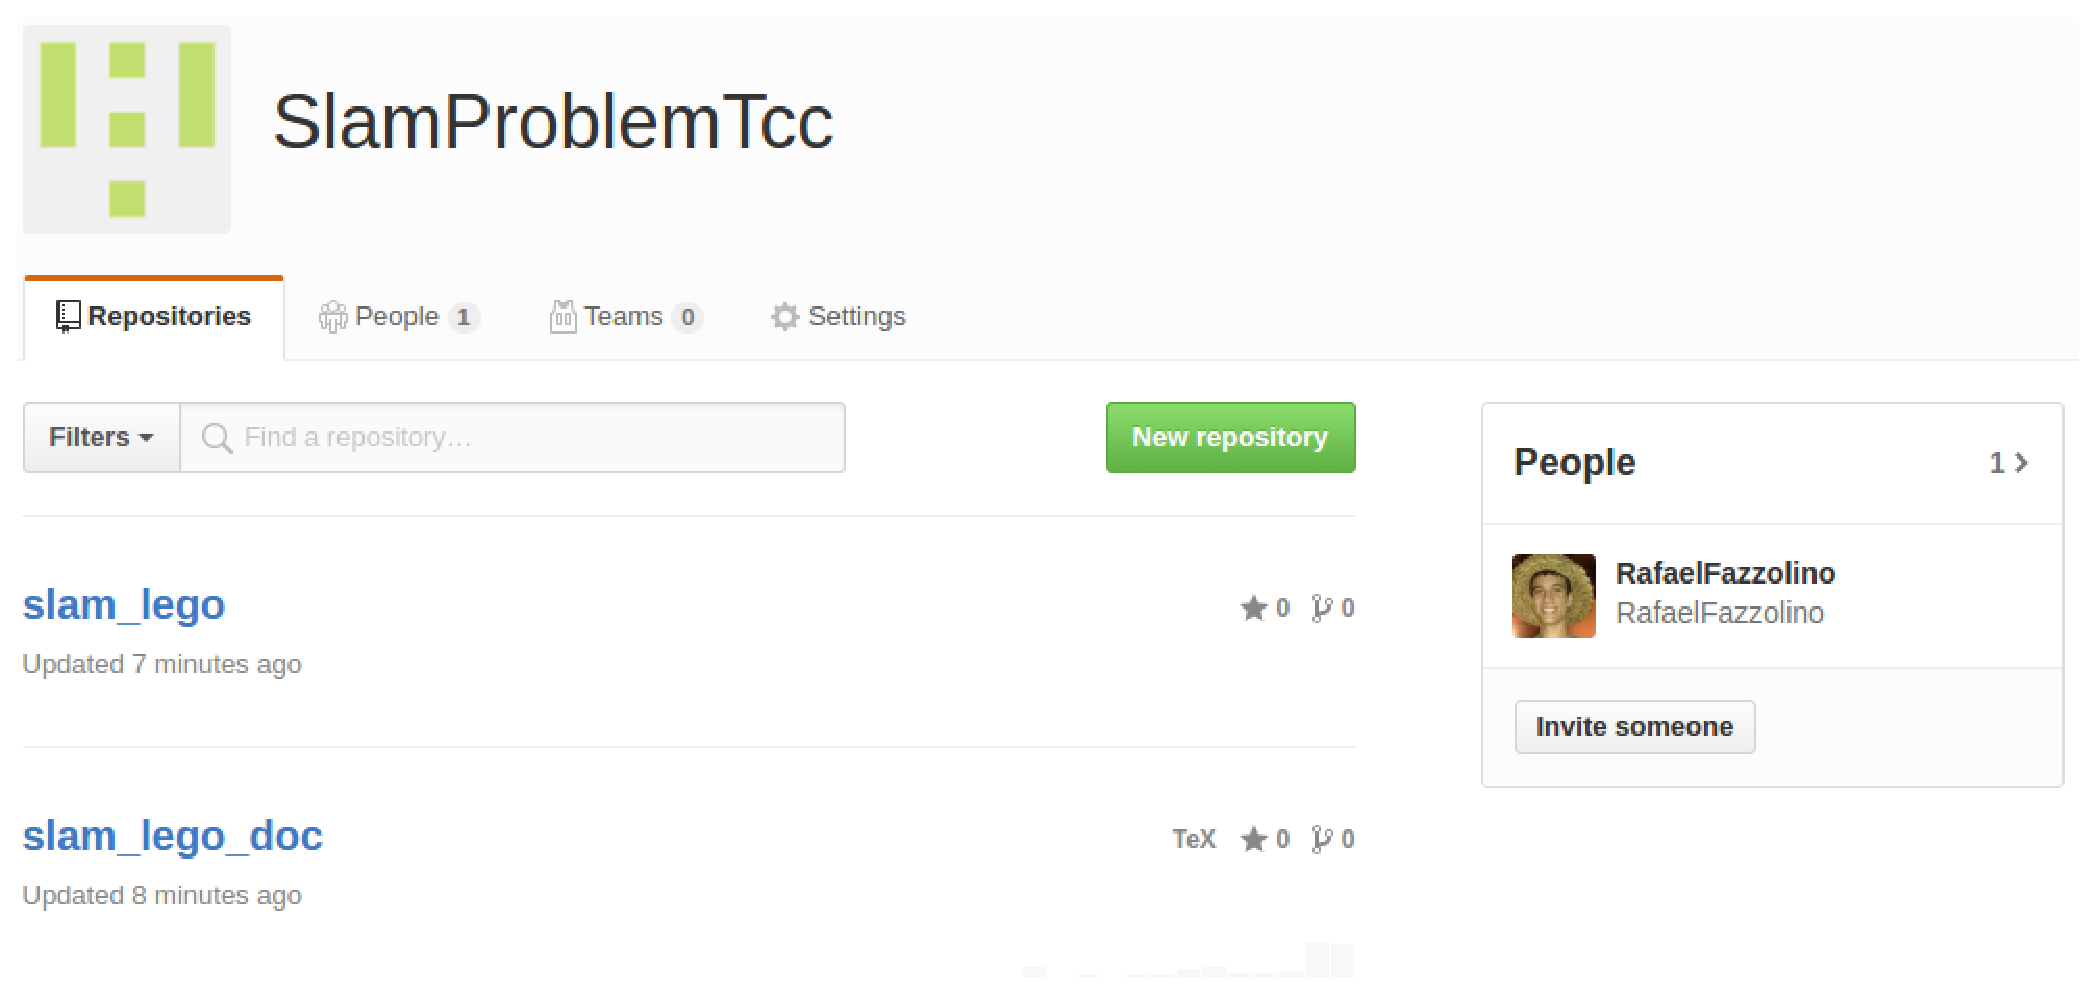
\includegraphics[scale=0.44]{figuras/github.eps}
			\caption[Página utilizada para versionamento do trabalho]{Página utilizada para versionamento do trabalho}
			\label{img:github}
		\end{figure}
	% subsection condução_do_trabalho (end)
	% subsection arquitetura_do_robô (end)
	
% section adaptação_e_implementação (end)

\section{Considerações parciais} % (fold)
\label{sec:considerações_parciais}

A proposta deste trabalho é baseada na identificação e adaptação de técnicas de resolução do problema de SLAM. Para isso foi realizada uma revisão sistemática para encontrar e registrar diferentes técnicas de SLAM utilizadas atualmente. Com a identificação destas técnicas, durante o TCC\_2, o foco do trabalho será adaptar algumas destas técnicas para o contexto simplificado da robótica educacional.

Este contexto simplipicado é baseado no kit de robótica Mindstorms, que, como já foi explicado, possui características bastante limitadas, como diversidade de sensores e capacidade de memória e processamento. A adaptação será implementada utilizando a linguagem Java, a partir da ferramenta \textit{leJOS NXJ}\footnote{http://www.lejos.org/nxj.php}.

Esta solução busca complementar uma sequência de soluções relacionadas à robótica educacional que vêm sendo desenvolvidas na Universidade de Brasília, como \cite{tccCarol} e \cite{tccRodrigo}. O \textit{framework} Traveller, desenvolvido por \cite{tccRodrigo}, será utilizado para navegação em ambientes já mapeados pelo algoritmo desenvolvido durante este trabalho. Desse modo, este trabalho tem como objetivo incorporar um módulo novo do \textit{framework}, possibilitando a construção de mapas e auto-localização nos mesmos.


% section considerações_parciais (end)